% ============================================================
% ECON 308 — International Economic Relations
% Lecture 4: Resources and Trade — The Heckscher-Ohlin Model
%            (Chapter 5)
% Fall 2026  |  Muhebullah Karimzada  |  UNBC
% ============================================================
\documentclass[aspectratio=169]{beamer}
\usepackage[utf8]{inputenc}
\usepackage[T1]{fontenc}
\usepackage{lmodern}
\usepackage{textcomp}

%% ── Theme and colours ───────────────────────────────────────
\usetheme{Madrid}
\setbeamertemplate{navigation symbols}{}
\setbeamercovered{transparent}
\setbeamertemplate{itemize items}[circle]
\setbeamertemplate{enumerate items}[default]
\setlength{\parskip}{0.15em}

\definecolor{UNBCDark}    {RGB}{0,74,37}
\definecolor{UNBCGold}    {RGB}{189,155,96}
\definecolor{SoftGray}    {RGB}{244,246,248}
\definecolor{AccentRed}   {RGB}{192,57,43}
\definecolor{AccentBlue}  {RGB}{41,98,255}
\definecolor{AccentTeal}  {RGB}{0,150,136}
\definecolor{AccentOrange}{RGB}{230,126,34}

\setbeamercolor{normal text}         {fg=black,bg=white}
\setbeamercolor{structure}           {fg=UNBCDark}
\setbeamercolor{title}               {fg=white,bg=UNBCDark}
\setbeamercolor{subtitle}            {fg=UNBCGold}
\setbeamercolor{frametitle}          {fg=white,bg=UNBCDark}
\setbeamercolor{block title}         {fg=white,bg=UNBCDark}
\setbeamercolor{block body}          {fg=black,bg=SoftGray}
\setbeamercolor{block title alerted} {fg=white,bg=AccentRed}
\setbeamercolor{block body alerted}  {fg=black,bg=SoftGray}
\setbeamercolor{item}                {fg=UNBCDark}
\setbeamercolor{alerted text}        {fg=AccentRed}
\setbeamercolor{author in head/foot} {fg=white,bg=UNBCDark}
\setbeamercolor{date in head/foot}   {fg=white,bg=UNBCDark}

%% ── Packages ────────────────────────────────────────────────
\usepackage{booktabs,multirow,array,amsmath,amssymb,bm,
            graphicx,adjustbox,tikz,pgfplots,tcolorbox,hyperref}
\tcbuselibrary{skins}
\pgfplotsset{compat=1.18}
\usetikzlibrary{arrows.meta,positioning,calc,shapes.geometric,
                decorations.pathreplacing}
\hypersetup{colorlinks=true,linkcolor=UNBCDark}

%% ── Footline ────────────────────────────────────────────────
\setbeamertemplate{headline}{}
\setbeamertemplate{footline}{%
  \leavevmode\hbox{%
  \begin{beamercolorbox}[wd=.78\paperwidth,ht=2.6ex,dp=1.0ex,
                         leftskip=1em]{author in head/foot}%
    \color{white}\textbf{ECON 308}\hspace{0.4em}%
    \textcolor{UNBCGold}{$\vert$}\hspace{0.4em}%
    International Economic Relations%
  \end{beamercolorbox}%
  \begin{beamercolorbox}[wd=.22\paperwidth,ht=2.6ex,dp=1.0ex,
                         rightskip=1em plus 1fil]{date in head/foot}%
    \color{white}\hfill\insertframenumber/\inserttotalframenumber%
  \end{beamercolorbox}}%
}

%% ── Custom tcolorboxes ──────────────────────────────────────
\newtcolorbox{insight}[1]{%
  colback=UNBCGold!12,colframe=UNBCGold!70!black,
  title={\small\bfseries #1},
  left=1mm,right=1mm,top=0.4mm,bottom=0.4mm,
  boxrule=0.5pt,arc=2mm}
\newtcolorbox{canadex}[1][Canadian Example]{%
  colback=AccentTeal!9,colframe=AccentTeal,
  title={\small\bfseries #1},
  left=1mm,right=1mm,top=0.4mm,bottom=0.4mm,
  boxrule=0.5pt,arc=2mm}
\newtcolorbox{discuss}{%
  colback=AccentBlue!8,colframe=AccentBlue,
  title={\small\bfseries Discussion},
  left=1mm,right=1mm,top=0.4mm,bottom=0.4mm,
  boxrule=0.5pt,arc=2mm}
\newtcolorbox{worked}{%
  colback=AccentOrange!8,colframe=AccentOrange,
  title={\small\bfseries Worked Example},
  left=1mm,right=1mm,top=0.4mm,bottom=0.4mm,
  boxrule=0.5pt,arc=2mm}
\newtcolorbox{varbox}{%
  colback=SoftGray,colframe=UNBCDark!40,
  left=1mm,right=1mm,top=0.4mm,bottom=0.4mm,
  boxrule=0.4pt,arc=2mm}

%% ── Figure helpers ──────────────────────────────────────────
\newcommand{\FIG}[1]{%
  \begin{center}%
  \includegraphics[width=\columnwidth,height=0.63\textheight,
                   keepaspectratio]{#1}%
  \end{center}}
\newcommand{\FIGS}[2][0.92]{%
  \begin{center}%
  \includegraphics[width=#1\columnwidth,height=0.63\textheight,
                   keepaspectratio]{#2}%
  \end{center}}

%% ── Metadata ────────────────────────────────────────────────
\title{\textbf{Resources and Trade: The Heckscher-Ohlin Model}}
\subtitle{{\large ECON 308\enspace International Economic
  Relations\enspace\textcolor{UNBCGold}{$|$}\enspace
  Chapter~5}}
\author{Muhebullah Karimzada}
\institute{School of Economics\\
           University of Northern British Columbia}
\date{Fall 2026}

% ============================================================
\begin{document}
% ============================================================

%% ─────────────────────────────────────────────────────────────
%% 1. TITLE
%% ─────────────────────────────────────────────────────────────
\begin{frame}[plain]
\titlepage
\end{frame}

%% ─────────────────────────────────────────────────────────────
%% 2. OPENING PUZZLE
%% ─────────────────────────────────────────────────────────────
\begin{frame}[shrink=10]{Opening Puzzle: Why Does Canada Export Oil to China?}
\begin{columns}[T]
\begin{column}{0.55\textwidth}
\begin{itemize}\small
  \item Canada and China use similar production
        technologies. The Ricardian model predicts
        \emph{little} trade between such countries.
  \item Yet Canada exports \textbf{oil, potash, and lumber}
        to China and imports \textbf{electronics and
        consumer goods} --- billions of dollars each year.
  \item \textbf{The puzzle}: if technology is the same,
        what drives such different trade patterns?
  \item \textbf{Answer}: factor \emph{endowments}.
        Canada has vast land and resources; China has
        abundant unskilled labour.
\end{itemize}
\vspace{0.2em}
\begin{insight}{Today's Model}
\small The \textbf{Heckscher-Ohlin model} shows how
differences in factor endowments generate comparative
advantage even with identical technology.
\end{insight}
\end{column}
\begin{column}{0.42\textwidth}
\begin{adjustbox}{max width=\columnwidth}
\begin{tabular}{lll}
\toprule
\textbf{Country} & \textbf{Abundant factor} & \textbf{Main exports}\\
\midrule
Canada & Land, resources & Oil, wheat, lumber\\
China & Unskilled labour & Electronics, textiles\\
USA & Capital, skills & Aircraft, software\\
Germany & Skilled labour & Machinery, cars\\
Bangladesh & Unskilled labour & Garments\\
\bottomrule
\end{tabular}
\end{adjustbox}
\vspace{0.4em}
\begin{varbox}
\small\textbf{Ricardian vs.\ H-O:}\\[0.2em]
Ricardian: technology differences\\
H-O: factor endowment differences\\[0.2em]
Both generate comparative advantage
but through different mechanisms.
\end{varbox}
\end{column}
\end{columns}
\end{frame}

%% ─────────────────────────────────────────────────────────────
%% 3. WHERE WE ARE
%% ─────────────────────────────────────────────────────────────
\begin{frame}[shrink=7]{Where We Are: The Model Family}
\begin{columns}[T]
\begin{column}{0.52\textwidth}
\begin{itemize}\small
  \item \textbf{Ch.~2} (Lecture~1): Trade facts and the
        gravity model --- \emph{who} trades with whom.
  \item \textbf{Ch.~3} (Lecture~2): \emph{Why} trade?
        Technology differences (Ricardian). Everyone gains.
  \item \textbf{Ch.~4} (Lecture~3): \emph{Who} wins and
        loses? Short-run specificity. Some factors lose.
  \item \textbf{Ch.~5} (today): Long-run H-O model.
        Both factors mobile. \emph{What} drives trade when
        technology is the same everywhere?
  \item \textbf{Ch.~6} (next): The Standard Trade Model
        --- a general synthesis.
\end{itemize}
\vspace{0.4em}
\begin{varbox}
\footnotesize\textbf{Short run vs.\ long run:}\\[0.2em]
Ch.~4 (Specific Factors) = capital locked in sector.\\
Ch.~5 (H-O) = capital \emph{fully mobile} across sectors.\\[0.2em]
As time passes, SF $\longrightarrow$ H-O.
\end{varbox}
\end{column}
\begin{column}{0.45\textwidth}
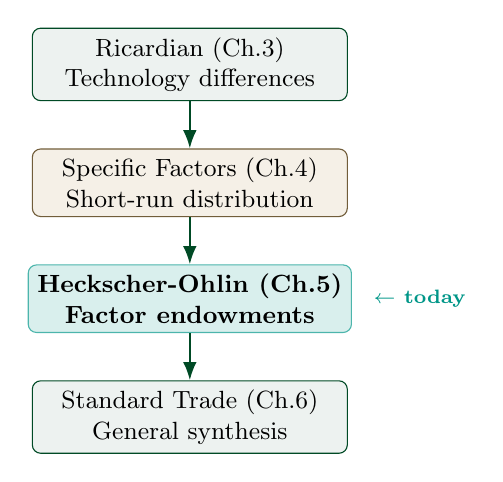
\begin{tikzpicture}[node distance=0.60cm,
  box/.style={draw=UNBCDark,fill=UNBCDark!7,rounded corners=3pt,
              minimum width=4.0cm,minimum height=0.60cm,
              align=center,font=\small}]
  \node[box](R){Ricardian (Ch.3)\\Technology differences};
  \node[box,below=of R,fill=UNBCGold!15,draw=UNBCGold!60!black]
       (SF){Specific Factors (Ch.4)\\Short-run distribution};
  \node[box,below=of SF,fill=AccentTeal!15,draw=AccentTeal!70,
        font=\small\bfseries]
       (HO){Heckscher-Ohlin (Ch.5)\\Factor endowments};
  \node[box,below=of HO](ST){Standard Trade (Ch.6)\\General synthesis};
  \draw[-{Latex},UNBCDark,thick](R)--(SF);
  \draw[-{Latex},UNBCDark,thick](SF)--(HO);
  \draw[-{Latex},UNBCDark,thick](HO)--(ST);
  \node[AccentTeal,font=\scriptsize\bfseries,right=0.15cm of HO]
       {$\leftarrow$ today};
\end{tikzpicture}
\end{column}
\end{columns}
\end{frame}

%% ─────────────────────────────────────────────────────────────
%% 4. LEARNING OBJECTIVES
%% ─────────────────────────────────────────────────────────────
\begin{frame}{Learning Objectives}
After this lecture you will be able to:
\begin{enumerate}\small
  \item Define \textbf{factor abundance} and \textbf{factor
        intensity}; state the Heckscher-Ohlin theorem.
  \item Derive cost-minimizing factor ratios from Cobb-Douglas
        technology and determine comparative advantage
        from factor endowments.
  \item Apply the \textbf{Stolper-Samuelson theorem} to identify
        winners and losers from trade in the long run.
  \item Explain the \textbf{magnification effect} and show why
        real factor gains/losses exceed the price change.
  \item State the \textbf{Factor Price Equalization} theorem
        and explain why it fails empirically.
  \item Apply the \textbf{Rybczynski theorem} to predict how
        factor accumulation alters the production mix.
  \item Connect the Rybczynski theorem to \textbf{Dutch Disease}
        and Canadian immigration policy.
  \item Evaluate the \textbf{Leontief Paradox} and the
        trade-versus-technology debate on wage inequality.
\end{enumerate}
\begin{block}{}
\small Krugman, Obstfeld \& Melitz, \textit{International
Economics}, 12th ed., Chapter~5.
\end{block}
\end{frame}

%% ═══════════════════════════════════════════════════════════
%%  PART 1 — MODEL SETUP
%% ═══════════════════════════════════════════════════════════

%% ─────────────────────────────────────────────────────────────
%% 5. THE 2×2×2 FRAMEWORK
%% ─────────────────────────────────────────────────────────────
\begin{frame}[shrink=12]{The 2$\times$2$\times$2 Framework}
\begin{columns}[T]
\begin{column}{0.53\textwidth}
\textbf{The H-O model assumes:}
\begin{itemize}\small
  \item \textbf{2 countries}: Home ($H$), Foreign ($F$).
  \item \textbf{2 goods}: Computers (capital-intensive),
        Textiles (labour-intensive).
  \item \textbf{2 factors}: Capital $K$ and Labour $L$
        --- \emph{both fully mobile} across sectors (long run).
  \item \textbf{Same technology}: identical production
        functions in both countries.
  \item \textbf{Identical homothetic preferences}.
  \item \textbf{Perfect competition} everywhere.
\end{itemize}
\vspace{0.2em}
\begin{insight}{The Single Difference}
\small The \emph{only} difference is factor endowments:
$(K/L)_H \neq (K/L)_F$. This alone drives trade.
\end{insight}
\end{column}
\begin{column}{0.44\textwidth}
\begin{varbox}
\small\textbf{Variable list:}\\[0.2em]
$K, L$ \quad= capital and labour (Home)\\
$K^*, L^*$ = capital and labour (Foreign)\\
$a_{KX}, a_{LX}$ = K and L per unit of $X$\\
$a_{KY}, a_{LY}$ = K and L per unit of $Y$\\
$w$ = wage rate\\
$r$ = rental rate of capital\\
$P_X, P_Y$ = goods prices (world)\\[0.4em]
\textbf{Key ratio:}\\
$(K/L)_H > (K/L)_F$\\
$\Rightarrow$ Home is \textbf{capital-abundant}\\
$\Rightarrow$ Foreign is \textbf{labour-abundant}
\end{varbox}
\end{column}
\end{columns}
\end{frame}

%% ─────────────────────────────────────────────────────────────
%% 6. FACTOR ABUNDANCE
%% ─────────────────────────────────────────────────────────────
\begin{frame}[shrink=5]{Factor Abundance: Relative, Not Absolute}
\begin{columns}[T]
\begin{column}{0.53\textwidth}
\begin{block}{Definition: Factor Abundance}
Country $H$ is \textbf{capital-abundant} relative to
country $F$ if:
\[\frac{K_H}{L_H} > \frac{K_F}{L_F}\]
It does \emph{not} matter that $H$ might have fewer total
workers or less capital than $F$ in absolute terms.
\end{block}
\vspace{0.4em}
\textbf{Key insight}: abundance is always \emph{relative}.
\begin{itemize}\small
  \item Canada has fewer workers than China, but Canada
        has far more capital and natural resources per
        worker.
  \item Bangladesh has fewer workers than Germany, but
        Bangladesh's labour-to-capital ratio is much
        higher.
\end{itemize}
\end{column}
\begin{column}{0.44\textwidth}
\begin{adjustbox}{max width=\columnwidth}
\begin{tabular}{lccc}
\toprule
\textbf{Country} & $K$ & $L$ & $K/L$\\
\midrule
Canada (Home) & 600 & 300 & \textbf{2.0} \\
Mexico (Foreign) & 300 & 600 & \textbf{0.5} \\
\bottomrule
\end{tabular}
\end{adjustbox}
\vspace{0.5em}
\begin{varbox}
\small Canada has \textbf{twice} the capital per worker
as Mexico, even though Mexico has \textbf{twice} the
total labour.\\[0.3em]
$\Rightarrow$ Canada is \textbf{capital-abundant}.\\
$\Rightarrow$ Mexico is \textbf{labour-abundant}.\\[0.3em]
These are the numbers from Tutorial~1 --- we will
return to them in our worked example.
\end{varbox}
\end{column}
\end{columns}
\end{frame}

%% ─────────────────────────────────────────────────────────────
%% 7. FACTOR INTENSITY
%% ─────────────────────────────────────────────────────────────
\begin{frame}[shrink=12]{Factor Intensity: The Other Key Concept}
\begin{columns}[T]
\begin{column}{0.53\textwidth}
\begin{block}{Definition: Factor Intensity}
\small Good $X$ is \textbf{capital-intensive} relative to $Y$
if at \emph{any} factor price ratio $w/r$:
$\;K_X/L_X > K_Y/L_Y$\\
(Holds for all $w/r$ --- no factor intensity reversals.)
\end{block}
\vspace{0.2em}
\textbf{Cobb-Douglas cost minimization:}
\[\frac{K_i}{L_i} = \frac{\alpha_i}{1-\alpha_i}\cdot\frac{w}{r}\]
Computers ($\alpha_X=0.6$): $K/L = 1.5\,(w/r)$\\
Textiles ($\alpha_Y=0.3$): $K/L = 0.43\,(w/r)$\\[0.1em]
\small Computers always use more capital per worker.
\end{column}
\begin{column}{0.44\textwidth}
\begin{adjustbox}{max width=\columnwidth}
\begin{tabular}{lcc}
\toprule
\textbf{Industry} & $K/L$ ratio & Capital-int.?\\
\midrule
Semiconductors & Very high & \textcolor{AccentTeal}{\checkmark}\\
Aircraft & High & \textcolor{AccentTeal}{\checkmark}\\
Auto assembly & Medium & \textcolor{AccentTeal}{\checkmark}\\
Forestry & Medium-low & Depends\\
Apparel/textiles & Low & \textcolor{AccentRed}{$\times$}\\
Call centres & Very low & \textcolor{AccentRed}{$\times$}\\
\bottomrule
\end{tabular}
\end{adjustbox}
\vspace{0.4em}
\begin{insight}{Intuition}
A semiconductor fab needs expensive equipment
and few workers. A garment factory needs many
sewing operators and little machinery. This
\emph{persistent} difference in capital-per-worker
is what makes H-O work.
\end{insight}
\end{column}
\end{columns}
\end{frame}

%% ─────────────────────────────────────────────────────────────
%% 8. THE H-O THEOREM
%% ─────────────────────────────────────────────────────────────
\begin{frame}[shrink=13]{The Heckscher-Ohlin Theorem}
\begin{columns}[T]
\begin{column}{0.53\textwidth}
\begin{block}{H-O Theorem (Heckscher 1919; Ohlin 1933)}
A country \textbf{exports} the good that uses its
\textbf{abundant factor} intensively and \textbf{imports}
the good that uses its \textbf{scarce factor} intensively.
\end{block}
\vspace{0.4em}
\textbf{The mechanism (step by step):}
\begin{enumerate}\small
  \item Home is capital-abundant: $(K/L)_H > (K/L)_F$.
  \item Abundance of capital $\Rightarrow$ capital is
        relatively cheap in Home: $(r/w)_H < (r/w)_F$.
  \item Cheap capital $\Rightarrow$ computers
        (capital-intensive) are \emph{cheaper to produce}
        in Home.
  \item Lower relative cost $\Rightarrow$ Home has
        \textbf{comparative advantage in computers}.
  \item Home exports computers; Foreign exports textiles.
\end{enumerate}
\end{column}
\begin{column}{0.44\textwidth}
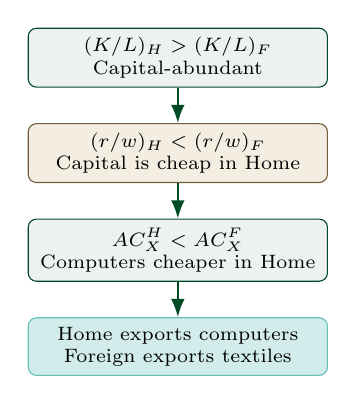
\begin{tikzpicture}[node distance=0.45cm,
  box/.style={draw=UNBCDark,fill=UNBCDark!7,rounded corners=3pt,
              minimum width=3.8cm,minimum height=0.52cm,
              align=center,font=\scriptsize}]
  \node[box](A){$(K/L)_H > (K/L)_F$\\Capital-abundant};
  \node[box,below=of A,fill=UNBCGold!18,draw=UNBCGold!60!black]
       (B){$(r/w)_H < (r/w)_F$\\Capital is cheap in Home};
  \node[box,below=of B](C){$AC_X^H < AC_X^F$\\Computers cheaper in Home};
  \node[box,below=of C,fill=AccentTeal!18,draw=AccentTeal!60]
       (D){Home exports computers\\Foreign exports textiles};
  \draw[-{Latex},UNBCDark,thick](A)--(B);
  \draw[-{Latex},UNBCDark,thick](B)--(C);
  \draw[-{Latex},UNBCDark,thick](C)--(D);
\end{tikzpicture}
\vspace{0.3em}
\begin{canadex}[Canada: H-O Confirmed]
\footnotesize
Canada (capital/resource abundant) exports\\
oil, potash, lumber, and wheat.\\[0.2em]
China (labour-abundant) exports garments,\\
electronics, and assembly goods.\\[0.2em]
The pattern matches H-O predictions.
\end{canadex}
\end{column}
\end{columns}
\end{frame}

%% ─────────────────────────────────────────────────────────────
%% 9. THE FACTOR BOX DIAGRAM
%% ─────────────────────────────────────────────────────────────
\begin{frame}[shrink=8]{The Factor Box: How Endowments Shape Production}
\begin{columns}[T]
\begin{column}{0.48\textwidth}
\textbf{The factor-allocation box} (Edgeworth box):
\begin{itemize}\small
  \item Width = total capital $\bar K$;
        Height = total labour $\bar L$.
  \item Allocation of $(K_X,L_X)$ to computers is read
        from bottom-left origin $O_X$.
  \item Remaining $(K_Y,L_Y)$ to textiles is read from
        top-right origin $O_Y$.
  \item At equilibrium, both sectors are on their
        \emph{isoquants} with the \emph{same} factor price
        ratio (parallel tangents).
\end{itemize}
\vspace{0.3em}
\textbf{Different endowments shift the box shape.}
A capital-abundant country's box is \emph{wider}
relative to its height --- pushing the equilibrium
allocation toward more computer production.
\end{column}
\begin{column}{0.49\textwidth}
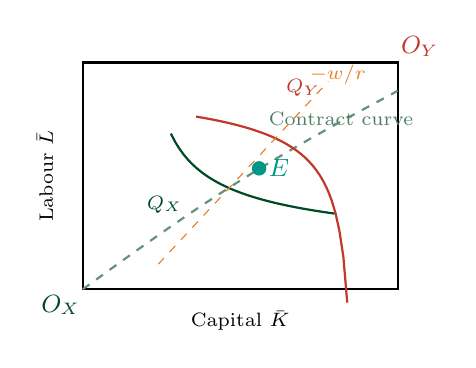
\begin{tikzpicture}[scale=0.80]
  % Box dimensions: width=5 (K), height=3.6 (L)
  \draw[thick](0,0) rectangle (5,3.6);
  % Origins
  \node[font=\small\bfseries,UNBCDark] at (-0.35,-0.25) {$O_X$};
  \node[font=\small\bfseries,AccentRed] at (5.35,3.85) {$O_Y$};
  % Axis labels
  \node[font=\scriptsize] at (2.5,-0.5) {Capital $\bar{K}$};
  \node[font=\scriptsize,rotate=90] at (-0.6,1.8) {Labour $\bar{L}$};
  % Contract curve (diagonal, slight bow)
  \draw[UNBCDark!60,thick,dashed,domain=0:5,samples=50]
       plot(\x,{0.63*\x + 0.15*sin(deg(3.14159*\x/5))});
  \node[UNBCDark!70,font=\scriptsize] at (4.1,2.7)
       {Contract curve};
  % Equilibrium point E
  \filldraw[AccentTeal](2.8,1.92) circle(3pt)
       node[right,font=\small]{$E$};
  % Isoquant for X (from O_X)
  \draw[UNBCDark,thick,domain=1.4:4.0,samples=40]
       plot(\x,{1.5/(\x-0.9)^0.5+0.35});
  \node[UNBCDark,font=\scriptsize] at (1.3,1.35){$Q_X$};
  % Isoquant for Y (from O_Y, drawn inverted)
  \draw[AccentRed,thick,domain=1.8:4.2,samples=40]
       plot(\x,{3.6 - 1.4/((5-\x-0.7)^0.5+0.05) + 0.0});
  \node[AccentRed,font=\scriptsize] at (3.5,3.2){$Q_Y$};
  % Factor price ratio lines at E (tangent)
  \draw[AccentOrange,thin,dashed](1.2,0.4)--(3.9,3.3);
  \node[AccentOrange,font=\scriptsize] at (4.05,3.4)
       {$-w/r$};
\end{tikzpicture}
\end{column}
\end{columns}
\end{frame}

%% ═══════════════════════════════════════════════════════════
%%  PART 2 — WORKED EXAMPLE
%% ═══════════════════════════════════════════════════════════

%% ─────────────────────────────────────────────────────────────
%% 10. WORKED EXAMPLE — SETUP
%% ─────────────────────────────────────────────────────────────
\begin{frame}[shrink=15]{Worked Example: Canada vs.\ Mexico}
\begin{worked}
\small\textbf{Technology} (identical in both countries):
$\;Q_C = K_C^{0.6}L_C^{0.4}$ (Computers, capital-intensive),
$\;Q_T = K_T^{0.3}L_T^{0.7}$ (Textiles, labour-intensive).\\[0.2em]
\textbf{Factor endowments:}
\begin{center}\small
\begin{tabular}{lcccc}
\toprule
\textbf{Country} & $K$ & $L$ & $K/L$ & \textbf{Abundant}\\
\midrule
Canada (Home) & 600 & 300 & 2.0 & Capital\\
Mexico (Foreign) & 300 & 600 & 0.5 & Labour\\
\bottomrule
\end{tabular}
\end{center}
\end{worked}
\vspace{0.2em}
\begin{columns}[T]
\begin{column}{0.50\textwidth}
\textbf{Step 1: Confirm factor intensity.}\\
Cobb-Douglas cost minimization:
\[\frac{K_i}{L_i} = \frac{\alpha_i}{1-\alpha_i}\cdot\frac{w}{r}\]
\end{column}
\begin{column}{0.47\textwidth}
At any $w/r$, computers use more capital:
\[\frac{K_C}{L_C} = 1.5\,\frac{w}{r} \;>\;
  \frac{K_T}{L_T} = 0.43\,\frac{w}{r}\]
\small$\Rightarrow$ $C$ is capital-intensive. \checkmark
\end{column}
\end{columns}
\end{frame}

%% ─────────────────────────────────────────────────────────────
%% 11. WORKED EXAMPLE — FACTOR PRICES AND COMPARATIVE ADVANTAGE
%% ─────────────────────────────────────────────────────────────
\begin{frame}[shrink=5]{Worked Example: Factor Prices and Trade Pattern}
\begin{columns}[T]
\begin{column}{0.50\textwidth}
\textbf{Step 2: Factor prices under autarky.}\\[0.3em]
Canada has abundant capital $\Rightarrow$ capital is
relatively cheap: $(w/r)_{Canada} = 1.5$.\\
Mexico has abundant labour $\Rightarrow$ labour is
relatively cheap: $(w/r)_{Mexico} = 3.0$.\\[0.4em]
\textbf{Step 3: K/L ratios in each country.}
\begin{center}
\begin{adjustbox}{max width=0.96\columnwidth}
\begin{tabular}{lcc}
\toprule
 & $(K/L)_C$ & $(K/L)_T$\\
\midrule
Canada ($w/r=1.5$) & $1.5\times1.5=2.25$ & $0.43\times1.5=0.65$\\
Mexico ($w/r=3.0$) & $1.5\times3.0=4.5$ & $0.43\times3.0=1.29$\\
\bottomrule
\end{tabular}
\end{adjustbox}
\end{center}
In both countries, computers remain more capital-intensive.
\end{column}
\begin{column}{0.47\textwidth}
\textbf{Step 4: Autarky relative prices.}\\[0.2em]
Cheap capital in Canada $\Rightarrow$ computers relatively
cheap in Canada:
\[(P_C/P_T)_{Canada} < (P_C/P_T)_{Mexico}\]
\textbf{Step 5: H-O prediction.}
\begin{varbox}
\small
$\Rightarrow$ Canada exports \textbf{computers}\\
$\Rightarrow$ Mexico exports \textbf{textiles}\\[0.3em]
If world price $(P_C/P_T)^W = 1.8$:\\
\begin{itemize}
  \item Canada's ToT improves from 1.2 to 1.8.
  \item Mexico's ToT deteriorates from 2.2 to 1.8.
  \item Both still gain overall (Ch.~3 logic).
\end{itemize}
\end{varbox}
\end{column}
\end{columns}
\end{frame}

%% ═══════════════════════════════════════════════════════════
%%  PART 3 — STOLPER-SAMUELSON THEOREM
%% ═══════════════════════════════════════════════════════════

%% ─────────────────────────────────────────────────────────────
%% 12. STOLPER-SAMUELSON: STATEMENT
%% ─────────────────────────────────────────────────────────────
\begin{frame}[shrink=7]{Stolper-Samuelson Theorem: Trade and Factor Returns}
\begin{columns}[T]
\begin{column}{0.53\textwidth}
\begin{block}{Stolper-Samuelson Theorem (1941)}
An increase in the \emph{relative price} of a good
raises the \textbf{real return} to the factor used
intensively in producing it and \textbf{lowers} the
real return to the other factor --- measured in terms
of \emph{both} goods.
\end{block}
\vspace{0.4em}
\textbf{Application to trade in Home (capital-abundant):}
\begin{itemize}\small
  \item Opening trade raises $P_X/P_Y$ in Home
        (computers become more valuable abroad).
  \item $\uparrow P_X \Rightarrow$ real return to
        capital \textbf{rises} (capital is intensive
        in computers).
  \item $\uparrow P_X \Rightarrow$ real wage
        \textbf{falls} (labour is intensive in textiles).
\end{itemize}
\end{column}
\begin{column}{0.44\textwidth}
\begin{alertblock}{Long-Run vs.\ Short-Run}
\small\textbf{Ch.~4 (Short run)}: labour's real wage
effect is \emph{ambiguous} --- it depends on which
good the worker consumes.\\[0.4em]
\textbf{Ch.~5 (Long run)}: the real wage falls
\emph{unambiguously} in terms of \emph{both} goods.
This is harsher!\\[0.4em]
Why harsher in the long run? Because capital can
move across sectors, intensifying the competition
for labour.
\end{alertblock}
\vspace{0.3em}
\begin{varbox}
\small\textbf{Remember:} This is real income, not
just nominal. Even if the nominal wage rises slightly,
it rises by \emph{less} than prices --- workers are
worse off in real terms.
\end{varbox}
\end{column}
\end{columns}
\end{frame}

%% ─────────────────────────────────────────────────────────────
%% 13. SS: THE MAGNIFICATION EFFECT
%% ─────────────────────────────────────────────────────────────
\begin{frame}{The Magnification Effect: Why Real Changes Exceed Price Changes}
\begin{columns}[T]
\begin{column}{0.52\textwidth}
\textbf{Intuition:} when $P_X$ rises, both sectors
compete harder for capital (the factor intensive in $X$).
Capital becomes scarce \emph{economy-wide} and its
return rises \emph{more than proportionally}.
Labour becomes relatively abundant and its return
falls in \emph{absolute} terms.\\[0.4em]
\textbf{Zero-profit conditions} pin wages and rentals:
\[\begin{aligned}
P_X &= a_{LX}\,w + a_{KX}\,r\\
P_Y &= a_{LY}\,w + a_{KY}\,r
\end{aligned}\]
A 10\% rise in $P_X$ requires $r$ to rise by
\emph{more} than 10\% (since $a_{KX}>0$ and $r$ must
absorb the full price increase after wages adjust).
\end{column}
\begin{column}{0.45\textwidth}
\begin{varbox}
\small\textbf{Magnification chain} (in \% changes):
\[\hat{r} > \hat{P}_X > 0 > \hat{P}_Y > \hat{w}\]
\textbf{Example:} $P_X$ rises 10\%, $P_Y$ unchanged.
\begin{itemize}
  \item $\hat{r} > 10\%$: capital gains more than
        the price rise.
  \item $\hat{w} < 0$: labour loses in \emph{absolute}
        terms (not just relative to computers).
\end{itemize}
\end{varbox}
\vspace{0.4em}
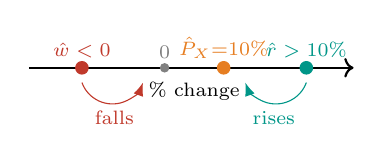
\begin{tikzpicture}[scale=0.75]
  \draw[thick,->](-0.3,0)--(5.2,0);
  \node[font=\scriptsize] at (2.5,-0.4){\% change};
  % Axis labels on number line
  \node[font=\scriptsize,below] at (0,-0.35){};
  % Markers
  \filldraw[AccentRed](0.6,0) circle(3pt)
       node[above,font=\scriptsize]{$\hat{w}<0$};
  \filldraw[gray](2.0,0) circle(2pt)
       node[above,font=\scriptsize]{$0$};
  \filldraw[AccentOrange](3.0,0) circle(3pt)
       node[above,font=\scriptsize]{$\hat{P}_X{=}10\%$};
  \filldraw[AccentTeal](4.4,0) circle(3pt)
       node[above,font=\scriptsize]{$\hat{r}>10\%$};
  \draw[-{Latex},AccentRed,thin](0.6,-0.25)arc[start angle=200,
       end angle=340,radius=0.55];
  \node[font=\scriptsize,AccentRed] at (1.15,-0.85){falls};
  \draw[-{Latex},AccentTeal,thin](4.4,-0.25)arc[start angle=-20,
       end angle=-160,radius=0.55];
  \node[font=\scriptsize,AccentTeal] at (3.85,-0.85){rises};
\end{tikzpicture}
\end{column}
\end{columns}
\end{frame}

%% ─────────────────────────────────────────────────────────────
%% 14. SS: WORKED NUMERICAL EXAMPLE
%% ─────────────────────────────────────────────────────────────
\begin{frame}[shrink=12]{Stolper-Samuelson: Worked Numerical Example}
\begin{worked}
\small\textbf{Given:} Computers ($X$): $a_{LX}=3$, $a_{KX}=6$.
Textiles ($Y$): $a_{LY}=4$, $a_{KY}=2$.
Prices: $P_X=10$, $P_Y=5$.
Find $w,r$; then $P_X$ rises to 11 (+10\%).
\end{worked}
\vspace{0.2em}
\begin{columns}[T]
\begin{column}{0.50\textwidth}
\textbf{Step 1: Initial equilibrium.}\\[0.1em]
Zero-profit: $\begin{cases}3w + 6r = 10\\4w + 2r = 5\end{cases}$\\[0.2em]
Solve: $\;\boxed{w\approx0.556,\quad r\approx0.722}$\\[0.4em]
\textbf{Step 2: After $P_X=11$ (+10\%).}\\[0.1em]
$\begin{cases}3w' + 6r' = 11\\4w' + 2r' = 5\end{cases}
\Rightarrow w'\approx0.333,\; r'\approx1.25$
\end{column}
\begin{column}{0.47\textwidth}
\textbf{Step 3: Real changes.}
\begin{center}\small
\begin{tabular}{lcc}
\toprule
& \textbf{Before} & \textbf{After}\\
\midrule
$P_X$ & 10 & 11 (+10\%)\\
$P_Y$ & 5 & 5 (0\%)\\
$w$ & 0.556 & 0.333 ($-$40\%)\\
$r$ & 0.722 & 1.25 (+73\%)\\
\bottomrule
\end{tabular}
\end{center}
\begin{insight}{Magnification Confirmed}
\small$\hat{r}=+73\%\gg\hat{P}_X=+10\%$\\
$\hat{w}=-40\%\ll\hat{P}_Y=0\%$
\end{insight}
\end{column}
\end{columns}
\end{frame}

%% ─────────────────────────────────────────────────────────────
%% 15. ACTIVE LEARNING: SS AND CANADIAN POLICY
%% ─────────────────────────────────────────────────────────────
\begin{frame}{Active Learning: Stolper-Samuelson and Canadian Trade Policy}
\begin{columns}[T]
\begin{column}{0.50\textwidth}
\begin{discuss}
\small
\textbf{Think--Pair--Share} (3 minutes):\\[0.3em]
Canada is capital-abundant and opens trade with
labour-abundant countries (China, Bangladesh).
\begin{enumerate}
  \item According to Stolper-Samuelson, which
        Canadian factor gains from this trade? Which
        loses?
  \item If trade lowers real wages in Canada, why
        do most Canadian economists \emph{still}
        support free trade?
  \item How does the \emph{Specific Factors} model
        (Ch.~4) give a different short-run prediction
        about Canadian wages?
\end{enumerate}
\end{discuss}
\end{column}
\begin{column}{0.47\textwidth}
\begin{canadex}[Canada--China Trade and Wages]
\small
After China joined WTO (2001), Canadian imports
from China surged.\\[0.3em]
SS prediction: Canadian workers in
labour-intensive sectors (textiles, apparel)
should see lower real wages.\\[0.3em]
\textbf{What happened?} Canadian manufacturing
employment fell, but wages held up --- partly
because displaced workers moved to services and
government safety nets absorbed shocks.\\[0.3em]
Key lesson: SS is a long-run model. Short-run
adjustment is painful even when long-run gains
are positive.
\end{canadex}
\end{column}
\end{columns}
\end{frame}

%% ═══════════════════════════════════════════════════════════
%%  PART 4 — FACTOR PRICE EQUALIZATION
%% ═══════════════════════════════════════════════════════════

%% ─────────────────────────────────────────────────────────────
%% 16. FPE THEOREM: STATEMENT
%% ─────────────────────────────────────────────────────────────
\begin{frame}[shrink=10]{Factor Price Equalization: Trade as a Substitute for Migration}
\begin{columns}[T]
\begin{column}{0.53\textwidth}
\begin{block}{Factor Price Equalization (Samuelson, 1948)}
Under free trade with \emph{identical technologies} and
\emph{no factor intensity reversals}, free trade in goods
\textbf{equalizes factor prices internationally} ---
even without any factor mobility.
\[w^H = w^F, \qquad r^H = r^F\]
\end{block}
\vspace{0.3em}
\textbf{Mechanism:}
\begin{enumerate}\small
  \item Free trade equalizes goods prices:
        $P_X^H = P_X^F$, $P_Y^H = P_Y^F$.
  \item Zero-profit conditions link goods prices
        to factor prices: same technology + same
        goods prices $\Rightarrow$ same $w$ and $r$.
  \item Trade in goods \emph{substitutes} for migration
        of factors.
\end{enumerate}
\end{column}
\begin{column}{0.44\textwidth}
\begin{alertblock}{Strong Prediction; Fails in Practice}
\small FPE says US wages should equal Chinese wages
under free trade. Clearly false!\\[0.4em]
\textbf{Why FPE fails:}
\begin{itemize}
  \item Technology \emph{differs} across countries.
  \item Trade barriers: tariffs and transport costs
        prevent full price equalization.
  \item Non-traded goods: services, housing.
  \item Factor intensity reversals.
  \item Countries may not produce the same goods
        (incomplete specialization).
\end{itemize}
\end{alertblock}
\end{column}
\end{columns}
\end{frame}

%% ─────────────────────────────────────────────────────────────
%% 17. FPE: INTUITION AND CANADIAN IMPLICATIONS
%% ─────────────────────────────────────────────────────────────
\begin{frame}[shrink=8]{FPE Intuition: Why Worry About Wage Equalization?}
\begin{columns}[T]
\begin{column}{0.53\textwidth}
\textbf{The logic of FPE:}\\[0.2em]
When Canada trades with Mexico, Mexican workers
do not need to move to Canada for their wages to
converge. Instead:
\begin{itemize}\small
  \item Canada imports textiles (labour-intensive)
        $\Rightarrow$ effectively ``importing'' Mexican
        labour indirectly.
  \item This reduces demand for Canadian unskilled
        labour $\Rightarrow$ Canadian wages fall toward
        Mexican wages.
  \item Mexico exports textiles $\Rightarrow$ demand
        for Mexican labour rises $\Rightarrow$ Mexican
        wages rise toward Canadian wages.
\end{itemize}
\vspace{0.3em}
\textbf{In practice:} wages converge only partially
and slowly due to technology differences, safety nets,
and labour market institutions.
\end{column}
\begin{column}{0.44\textwidth}
\begin{canadex}[CUSMA and Wage Pressure]
\small
After NAFTA (1994), Canadian low-skilled wages
did not fully equalize with Mexican wages.\\[0.3em]
\textbf{Why not?}
\begin{itemize}
  \item Canada has much higher productivity (technology
        gap offsets FPE).
  \item Services sector insulates workers from goods
        competition.
  \item Canada's generous minimum wages and transfers
        create a wage floor.
\end{itemize}
\textbf{Bottom line:} FPE is a useful benchmark.
Real-world convergence is partial and conditional
on technology convergence.
\end{canadex}
\end{column}
\end{columns}
\end{frame}

%% ═══════════════════════════════════════════════════════════
%%  PART 5 — RYBCZYNSKI THEOREM
%% ═══════════════════════════════════════════════════════════

%% ─────────────────────────────────────────────────────────────
%% 18. RYBCZYNSKI THEOREM: STATEMENT
%% ─────────────────────────────────────────────────────────────
\begin{frame}[shrink=12]{Rybczynski Theorem: Growth and Production Bias}
\begin{columns}[T]
\begin{column}{0.53\textwidth}
\begin{block}{Rybczynski Theorem (1955)}
At \textbf{constant goods prices}, an increase in one
factor endowment causes the output of the good using
that factor intensively to \textbf{expand} and the
output of the other good to \textbf{contract}.
\end{block}
\vspace{0.3em}
\textbf{Mechanism:}
\begin{enumerate}\small
  \item Capital stock grows ($K\uparrow$) at constant
        prices and therefore constant $w/r$.
  \item Each sector uses the same $K/L$ ratio (no
        factor intensity reversal; $w/r$ unchanged).
  \item But more capital must be absorbed. The only
        way: computers (capital-intensive) expand and
        \emph{release} labour that would otherwise
        go to textiles.
  \item Textiles \emph{contracts} because its labour
        supply shrinks.
\end{enumerate}
\end{column}
\begin{column}{0.44\textwidth}
\begin{varbox}
\small\textbf{Summary table:}\\[0.3em]
\begin{tabular}{lcc}
\toprule
\textbf{Endowment} & $Q_X$ (K-int.) & $Q_Y$ (L-int.)\\
\midrule
$K\uparrow$ & $\uparrow\uparrow$ & $\downarrow$\\
$L\uparrow$ & $\downarrow$ & $\uparrow\uparrow$\\
\bottomrule
\end{tabular}\\[0.4em]
$\uparrow\uparrow$ = super-proportional expansion
\end{varbox}
\vspace{0.4em}
\begin{insight}{Key Implication}
\small Growth reinforces comparative advantage.
A capital-accumulating country becomes
\emph{even more} specialised in capital-intensive
goods. Trade patterns persist and deepen.
\end{insight}
\end{column}
\end{columns}
\end{frame}

%% ─────────────────────────────────────────────────────────────
%% 19. RYBCZYNSKI: PPF DIAGRAM
%% ─────────────────────────────────────────────────────────────
\begin{frame}[shrink=5]{Rybczynski: Capital Accumulation Biases the PPF}
\begin{columns}[T]
\begin{column}{0.36\textwidth}
\textbf{Reading the diagram:}
\begin{itemize}\small
  \item \textcolor{UNBCDark}{\textbf{PPF}} (solid):
        before capital accumulation.
  \item \textcolor{AccentTeal}{\textbf{PPF$'$}}
        (dashed): after $K$ rises.
  \item Same price ratio (parallel orange lines)
        $\Rightarrow$ production shifts $A \to A'$.
  \item $Q_X$ (computers) \textbf{expands};
        $Q_Y$ (textiles) \textbf{contracts}.
  \item Income rises (outer line), but gain
        concentrates in computers.
\end{itemize}
\vspace{0.4em}
\small\textbf{The \textcolor{AccentRed}{Rybczynski arrow}}
$A \to A'$ has a \emph{negative} slope:
one good rises, the other falls simultaneously.
\end{column}
\begin{column}{0.61\textwidth}
% PPF:  y = 4.0*sqrt(1-(x/4.2)^2)
%   A at x=2.80: y=4.0*sqrt(0.556)=2.983
% PPF': y = 4.0*sqrt(1-(x/5.3)^2)
%   A'at x=3.96: y=4.0*sqrt(0.442)=2.659
% Isovalue slope -0.85: line1 y=5.363-0.85x; line2 y=6.025-0.85x
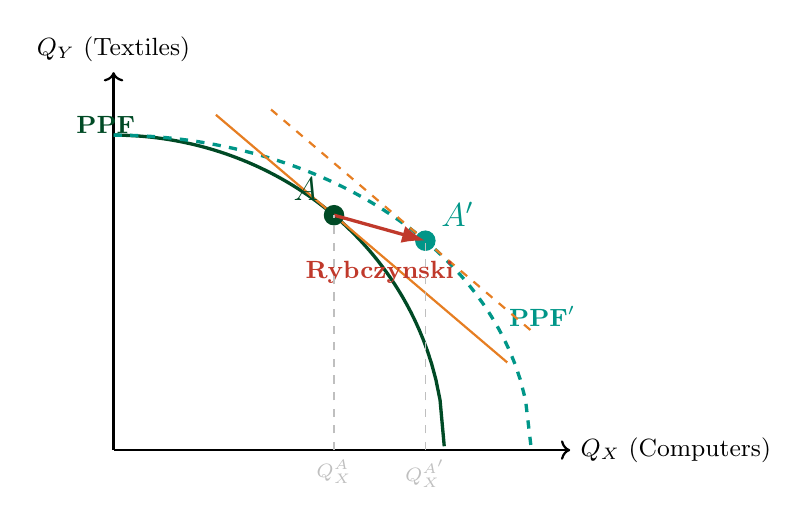
\begin{tikzpicture}
  \draw[->,thick](0,0)--(5.8,0)
       node[right,font=\small]{$Q_X$ (Computers)};
  \draw[->,thick](0,0)--(0,4.8)
       node[above,font=\small]{$Q_Y$ (Textiles)};
  %% Original PPF (dark green, solid)
  \draw[UNBCDark,very thick,domain=0:4.2,samples=80]
       plot(\x,{4.0*sqrt(max(0,1-(\x/4.2)^2))});
  \node[UNBCDark,font=\small\bfseries,anchor=south east]
       at (0.40,3.90){\textbf{PPF}};
  %% New PPF' (teal, dashed)
  \draw[AccentTeal,very thick,dashed,domain=0:5.3,samples=80]
       plot(\x,{4.0*sqrt(max(0,1-(\x/5.3)^2))});
  \node[AccentTeal,font=\small\bfseries,anchor=north west]
       at (4.90,1.95){\textbf{PPF$'$}};
  %% Isovalue line 1 (through A, slope -0.85)
  \draw[AccentOrange,thick](1.3,4.258)--(5.0,1.113);
  %% Isovalue line 2 (through A', same slope -0.85)
  \draw[AccentOrange,thick,dashed](2.0,4.325)--(5.3,1.520);
  %% Point A = (2.80, 2.983) — label above-left of dot
  \filldraw[UNBCDark](2.80,2.983) circle(3.5pt);
  \node[UNBCDark,font=\large\bfseries,anchor=south east]
       at (2.72,3.05){$A$};
  %% Point A' = (3.96, 2.659) — label above-right of dot
  \filldraw[AccentTeal](3.96,2.659) circle(3.5pt);
  \node[AccentTeal,font=\large\bfseries,anchor=south west]
       at (4.04,2.72){$A'$};
  %% Rybczynski arrow A -> A' (label below midpoint, well clear)
  \draw[-{Latex},AccentRed,very thick](2.80,2.983)--(3.96,2.659);
  \node[AccentRed,font=\small\bfseries,anchor=north]
       at (3.38,2.52){Rybczynski};
  %% Vertical dashed guides to x-axis
  \draw[dashed,gray!50,thin](2.80,0)
       node[below,font=\scriptsize]{$Q_X^A$}--(2.80,2.983);
  \draw[dashed,gray!50,thin](3.96,0)
       node[below,font=\scriptsize]{$Q_X^{A'}$}--(3.96,2.659);
\end{tikzpicture}
\end{column}
\end{columns}
\end{frame}

%% ─────────────────────────────────────────────────────────────
%% 20. DUTCH DISEASE: RYBCZYNSKI IN CANADA
%% ─────────────────────────────────────────────────────────────
\begin{frame}[shrink=5]{Dutch Disease: Rybczynski Applied to Canada}
\begin{columns}[T]
\begin{column}{0.53\textwidth}
\textbf{Dutch Disease} occurs when a resource boom
draws factors out of manufacturing, causing
manufacturing to \emph{contract}.
\begin{enumerate}\small
  \item \textbf{Resource discovery / price boom}: oil
        prices rise, making Alberta oil sands
        investment highly profitable.
  \item \textbf{Capital flows in}: $K$ in the resource
        sector rises.
  \item \textbf{Rybczynski}: resource output expands;
        manufacturing output contracts (at constant
        goods prices).
  \item \textbf{Exchange rate}: higher export revenues
        appreciate the CAD, making manufactured exports
        \emph{even less} competitive.
  \item \textbf{Double squeeze} on Ontario: higher
        factor costs + stronger CAD.
\end{enumerate}
\end{column}
\begin{column}{0.44\textwidth}
\begin{canadex}[Alberta Oil Sands, 2002--2014]
\small
\textbf{Oil investment surge}: oil sands capital
spending rose from \$3B/yr to \$30B/yr.\\[0.2em]
\textbf{Manufacturing response}: Ontario
manufacturing employment fell from 1.0M (2002)
to 0.72M (2014) --- a 28\% drop.\\[0.2em]
\textbf{Exchange rate}: CAD rose to parity with
USD by 2007, then above parity 2009--2013.\\[0.2em]
\textbf{Named after}: Netherlands, whose North Sea
gas discovery (1959) devastated Dutch manufacturing
by 1970s.\\[0.2em]
\textbf{Key insight}: structural policy cannot
easily offset Rybczynski-driven resource booms.
\end{canadex}
\end{column}
\end{columns}
\end{frame}

%% ─────────────────────────────────────────────────────────────
%% 21. RYBCZYNSKI AND IMMIGRATION
%% ─────────────────────────────────────────────────────────────
\begin{frame}[shrink=15]{Rybczynski and Immigration: Canada's Labour Supply}
\begin{columns}[T]
\begin{column}{0.53\textwidth}
\textbf{Canada's immigration rate} is among the
highest in the OECD --- over 400,000 permanent
residents per year since 2022.\\[0.4em]
\textbf{Rybczynski predicts:}
\begin{itemize}\small
  \item Immigration raises the labour supply:
        $L\uparrow$.
  \item At constant goods prices, output of
        labour-intensive goods expands; output of
        capital-intensive goods contracts.
  \item Canada's labour-intensive sector
        (services, agriculture) expands relative
        to capital-intensive manufacturing.
\end{itemize}
\vspace{0.3em}
\begin{insight}{The Immigration--FPE Connection}
\small FPE says trade substitutes for migration.
If trade already partially equalized wages,
immigration should have \emph{smaller} wage
effects than a closed-economy model would
predict.
\end{insight}
\end{column}
\begin{column}{0.44\textwidth}
\begin{discuss}
\small
\textbf{Discussion question:}\\[0.3em]
The Rybczynski theorem says that high immigration
($L\uparrow$) should increase output of
labour-intensive goods but \emph{reduce} output
of capital-intensive goods.\\[0.3em]
\begin{enumerate}
  \item Is this a good argument \emph{against}
        immigration?
  \item Does the theorem say anything about the
        \emph{wage effect} on existing workers?
        (Hint: see SS theorem.)
  \item Why might capital accumulation
        \emph{accompany} immigration, moderating
        the Rybczynski effect?
\end{enumerate}
\end{discuss}
\end{column}
\end{columns}
\end{frame}

%% ═══════════════════════════════════════════════════════════
%%  PART 6 — EMPIRICS AND THE LEONTIEF PARADOX
%% ═══════════════════════════════════════════════════════════

%% ─────────────────────────────────────────────────────────────
%% 22. THE LEONTIEF PARADOX
%% ─────────────────────────────────────────────────────────────
\begin{frame}[shrink=15]{The Leontief Paradox: Testing H-O}
\begin{columns}[T]
\begin{column}{0.53\textwidth}
\textbf{Leontief (1953)} tested H-O with 1947 US data.\\[0.2em]
\textbf{H-O prediction:} US is capital-abundant $\Rightarrow$
exports should be capital-intensive.\\[0.2em]
\textbf{Paradoxical finding:}
\begin{itemize}\small
  \item US exports were \textbf{labour-intensive}.
  \item US imports were \textbf{30\% more capital-intensive}.
  \item US appeared to be a \emph{labour-abundant}
        exporter --- opposite of H-O!
\end{itemize}
\vspace{0.2em}
\small The paradox shook confidence in H-O for decades.
\end{column}
\begin{column}{0.44\textwidth}
\begin{varbox}
\small\textbf{Proposed resolutions:}\\[0.3em]
\textbf{1. Human capital}: US exports embody
skilled labour; physical capital/labour ratios
miss this.\\[0.2em]
\textbf{2. Technology gap}: US comparative advantage
is in technology, not physical capital per se.\\[0.2em]
\textbf{3. Tariff structure}: US tariffs protected
labour-intensive industries.\\[0.2em]
\textbf{4. Demand bias}: US consumers prefer
capital-intensive goods more than foreigners do.
\end{varbox}
\vspace{0.3em}
\begin{insight}{Modern Verdict}
\small Trefler (1995): when human capital and
productivity differences are accounted for,
H-O performs much better. The ``missing trade''
puzzle largely resolves.
\end{insight}
\end{column}
\end{columns}
\end{frame}

%% ─────────────────────────────────────────────────────────────
%% 23. MODERN EVIDENCE: MULTI-FACTOR H-O
%% ─────────────────────────────────────────────────────────────
\begin{frame}[shrink=5]{Modern Evidence: Beyond Physical Capital}
\begin{columns}[T]
\begin{column}{0.50\textwidth}
\textbf{Key insight from empirical research:}
The H-O model works better when we broaden
the definition of factors.\\[0.4em]
\textbf{Three-factor H-O model:}
\begin{itemize}\small
  \item \textbf{Physical capital} $K$: machinery,
        buildings, equipment.
  \item \textbf{Human capital} $H$: education,
        training, skills.
  \item \textbf{Natural resources} $N$: land,
        oil, minerals, forests.
\end{itemize}
\vspace{0.3em}
With all three factors:
\begin{itemize}\small
  \item US: abundant in $K$ and $H$
        $\Rightarrow$ exports aircraft, software,
        pharmaceuticals.
  \item Canada: abundant in $N$ (and $K$)
        $\Rightarrow$ exports resources plus
        financial services.
  \item China: abundant in $L$ (unskilled)
        $\Rightarrow$ exports manufactures.
\end{itemize}
\end{column}
\begin{column}{0.47\textwidth}
\begin{adjustbox}{max width=\columnwidth}
\begin{tabular}{lccc}
\toprule
& \textbf{Physical}$K$ & \textbf{Human}$H$ &
  \textbf{Natural}$N$\\
\midrule
Canada & Medium & High & \textbf{Very high}\\
USA & \textbf{High} & \textbf{High} & Medium\\
China & Medium & Low--med. & Low\\
Germany & High & \textbf{High} & Low\\
Bangladesh & Low & Low & Low\\
\midrule
\textbf{Main export} & Machinery & Soft./pharma &
  Resources\\
\bottomrule
\end{tabular}
\end{adjustbox}
\vspace{0.4em}
\begin{canadex}[Canada's Multi-Factor Abundance]
\small Canada's comparative advantage in natural
resources is overwhelming. For every unit of natural
capital per worker, Canada ranks among the top 3
globally. This explains the persistence of resource
exports despite a high wage level.
\end{canadex}
\end{column}
\end{columns}
\end{frame}

%% ═══════════════════════════════════════════════════════════
%%  PART 7 — TRADE AND WAGE INEQUALITY
%% ═══════════════════════════════════════════════════════════

%% ─────────────────────────────────────────────────────────────
%% 24. TRADE AND INEQUALITY: THE DEBATE
%% ─────────────────────────────────────────────────────────────
\begin{frame}[shrink=15]{Trade and Wage Inequality: Two Explanations}
\begin{columns}[T]
\begin{column}{0.52\textwidth}
\textbf{Fact}: In rich countries, wage inequality
has risen sharply since the 1980s.\\[0.3em]
\textbf{Explanation 1 — Trade (Stolper-Samuelson):}
\begin{itemize}\small
  \item Trade with labour-abundant countries
        lowers demand for unskilled labour in
        capital-abundant countries.
  \item H-O predicts falling real wages for
        unskilled workers in the US and Canada.
\end{itemize}
\vspace{0.2em}
\textbf{Explanation 2 — Skill-Biased Tech Change (SBTC):}
\begin{itemize}\small
  \item Computers and automation displace
        routine/unskilled tasks.
  \item Raises relative demand for skilled workers.
  \item Works even in a closed economy.
\end{itemize}
\vspace{0.2em}
\textbf{Verdict:} Both contribute, but SBTC has
historically accounted for more of the rise.
\end{column}
\begin{column}{0.45\textwidth}
\begin{adjustbox}{max width=\columnwidth}
\begin{tabular}{lcc}
\toprule
\textbf{Factor} & \textbf{Trade} & \textbf{SBTC}\\
\midrule
Unskilled labour & Lose & Lose\\
Skilled labour & Gain & Gain\\
Capital owners & Gain & Gain\\
\midrule
\textbf{Mechanism} & SS theorem & Automation\\
\textbf{Scope} & Open economy & Any economy\\
\bottomrule
\end{tabular}
\end{adjustbox}
\vspace{0.4em}
\begin{insight}{Consensus (Autor et al.)}
\small Trade and SBTC are complements, not
rivals. SBTC raised skill premia everywhere.
The ``China shock'' (post-2001) shows trade
effects are larger than previously estimated,
especially for local labour markets.
\end{insight}
\end{column}
\end{columns}
\end{frame}

%% ─────────────────────────────────────────────────────────────
%% 25. THE CHINA SHOCK: MACRO CONNECTION
%% ─────────────────────────────────────────────────────────────
\begin{frame}[shrink=15]{The China Shock: Trade and Regional Unemployment}
\begin{columns}[T]
\begin{column}{0.52\textwidth}
\textbf{Autor, Dorn \& Hanson (2013)}: regional impact
of Chinese import competition after WTO accession (2001).\\[0.2em]
\textbf{Key findings:}
\begin{itemize}\small
  \item US zones exposed to Chinese competition saw
        lasting \emph{employment and wage declines}.
  \item Workers did \emph{not} easily relocate
        (H-O assumes mobile labour --- violated).
  \item Aggregate gains positive, but distribution
        highly unequal and geographically concentrated.
\end{itemize}
\vspace{0.2em}
\small\textbf{Policy}: free trade needs redistribution
mechanisms to be politically sustainable.
\end{column}
\begin{column}{0.45\textwidth}
\begin{canadex}[Canada's China Shock]
\footnotesize
Canada's resource exports to China \emph{grew}
(H-O: Canadian comparative advantage in resources).\\[0.2em]
Textile/apparel sector contracted sharply.\\[0.2em]
Strong safety net (EI) cushioned adjustment.\\[0.2em]
CUSMA preserved auto/aerospace via rules of origin.
\end{canadex}
\vspace{0.2em}
\begin{insight}{Macro Link}
\footnotesize Trade shocks affect regional unemployment
$\Rightarrow$ BoC rate decisions. The 2015
commodity/trade shock drove rates near zero
through 2015--2017.
\end{insight}
\end{column}
\end{columns}
\end{frame}

%% ─────────────────────────────────────────────────────────────
%% 26. CANADIAN WAGE INEQUALITY
%% ─────────────────────────────────────────────────────────────
\begin{frame}[shrink=5]{Canadian Wage Inequality: Trade and Technology}
\begin{columns}[T]
\begin{column}{0.52\textwidth}
\textbf{Canada's labour market, 1980--2025:}
\begin{itemize}\small
  \item Skill premium (university vs.\ high-school
        wages) rose by roughly 20--25 percentage
        points.
  \item Top-1\% income share rose from 8\% (1980)
        to 14\% (2015), then stabilized.
  \item Manufacturing employment share fell from
        20\% (1980) to 9\% (2022).
\end{itemize}
\vspace{0.2em}
\textbf{SS prediction}: trade with China/Bangladesh
should lower wages of unskilled Canadian workers.
\begin{itemize}\small
  \item Partial confirmation: textile/apparel wages
        fell relative to economy-wide wages.
  \item But: Canadian minimum wage laws and collective
        agreements moderated the effect.
  \item SBTC also important: resource boom raised
        returns to capital and skilled engineers.
\end{itemize}
\end{column}
\begin{column}{0.45\textwidth}
\begin{canadex}[CUSMA and Skilled Labour]
\small Under CUSMA, Canadian capital-intensive sectors
(aerospace, automotive, financial services) are
largely protected through rules of origin.\\[0.3em]
Result: Canada retains comparative advantage in
capital- and skill-intensive sectors within North
America, while losing labour-intensive sectors to
global competition.\\[0.3em]
\textbf{SS in CUSMA context}: CUSMA raises
$P_X$ (capital-intensive goods) for Canada
$\Rightarrow$ SS predicts capital and skills gain;
unskilled labour faces competition from Mexico.
\end{canadex}
\end{column}
\end{columns}
\end{frame}

%% ═══════════════════════════════════════════════════════════
%%  PART 8 — POLICY, MACRO CONNECTIONS, AND SYNTHESIS
%% ═══════════════════════════════════════════════════════════

%% ─────────────────────────────────────────────────────────────
%% 27. POLICY APPLICATION: H-O AND TRADE AGREEMENTS
%% ─────────────────────────────────────────────────────────────
\begin{frame}[shrink=15]{Policy Application: H-O and the Design of Trade Agreements}
\begin{columns}[T]
\begin{column}{0.53\textwidth}
\textbf{H-O has direct implications for trade
agreement design:}\\[0.4em]
\textbf{1. Who pushes for free trade?}
\begin{itemize}\small
  \item Owners of the abundant factor lobby
        \emph{for} trade (SS: they gain).
  \item Owners of the scarce factor lobby
        \emph{against} trade (SS: they lose).
\end{itemize}
\vspace{0.2em}
\textbf{2. CUSMA rules of origin:}
\begin{itemize}\small
  \item Canadian auto sector: requires 75\% North
        American content, protecting capital-intensive
        assembly.
  \item Mexican textiles: preferential tariff access
        to Canada, leveraging labour abundance.
\end{itemize}
\vspace{0.2em}
\textbf{3. CPTPP and resource endowments:}
\begin{itemize}\small
  \item Canada's abundant natural resources gain
        tariff-free access to Japan and Vietnam.
  \item Consistent with H-O: trade agreement unlocks
        endowment-based gains.
\end{itemize}
\end{column}
\begin{column}{0.44\textwidth}
\begin{canadex}[Canadian Dairy: SS in Action]
\small Supply management (dairy, poultry, eggs)
maintains high domestic prices via
tariff-rate quotas.\\[0.2em]
\textbf{H-O interpretation:} Canada is not
land-abundant enough to compete with New Zealand
or Australia in dairy on world markets.\\[0.2em]
\textbf{SS interpretation:} Dairy sector owners
(capital- and land-specific) lobby \emph{against}
trade because import competition would drive
down returns to dairy capital.\\[0.2em]
\textbf{Redistribution cost:} Canadian consumers
pay $\approx$\$2B/year more for dairy products
(C.D.\ Howe Institute, 2019).
\end{canadex}
\end{column}
\end{columns}
\end{frame}

%% ─────────────────────────────────────────────────────────────
%% 28. MACROECONOMIC CONNECTIONS
%% ─────────────────────────────────────────────────────────────
\begin{frame}[shrink=15]{Macroeconomic Connections: H-O and the Canadian Economy}
\begin{columns}[T]
\begin{column}{0.50\textwidth}
\textbf{1. Terms of trade and national income:}
\begin{itemize}\small
  \item Trade raises $P_X/P_Y$ for exporter (Canada
        in computers; Saudi Arabia in oil).
  \item Rise in ToT $\Rightarrow$ real national
        income rises (import more with same exports).
  \item Canadian commodity boom 2003--2014: oil
        prices tripled $\Rightarrow$ ToT improved
        $\Rightarrow$ real income up in Alberta.
\end{itemize}
\vspace{0.3em}
\textbf{2. Factor accumulation and growth:}
\begin{itemize}\small
  \item Rybczynski: capital accumulation biases
        production toward capital-intensive goods.
  \item Amplifies comparative advantage over time.
  \item Connects to Standard Trade Model (Ch.~6):
        export-biased growth and terms-of-trade
        effects.
\end{itemize}
\end{column}
\begin{column}{0.47\textwidth}
\textbf{3. Trade, wages, and monetary policy:}
\begin{varbox}
\small\textbf{The chain for Canada:}\\[0.2em]
Trade $\uparrow$ capital return
$\xrightarrow{\text{SS}}$
higher $r$ in resource-rich sectors
$\xrightarrow{\text{investment}}$
Rybczynski: resource output $\uparrow$,
manufacturing $\downarrow$
$\xrightarrow{\text{exchange rate}}$
CAD appreciates
$\xrightarrow{\text{further}}$
manufactured exports $\downarrow$
$\xrightarrow{\text{Bank of Canada}}$
one interest rate must serve two
diverging sectors
\end{varbox}
\vspace{0.3em}
\begin{insight}{One-Rate Problem}
\small Canada's single monetary policy cannot
simultaneously prevent inflation in booming
Alberta and stimulate depressed Ontario ---
a recurring tension in Canadian macro policy.
\end{insight}
\end{column}
\end{columns}
\end{frame}

%% ─────────────────────────────────────────────────────────────
%% 29. ACTIVE LEARNING: THE FOUR THEOREMS
%% ─────────────────────────────────────────────────────────────
\begin{frame}[shrink=15]{Active Learning: Applying the Four Theorems}
\begin{columns}[T]
\begin{column}{0.50\textwidth}
\begin{discuss}
\small\textbf{Apply each theorem to Canada.
Work in pairs (4 minutes).}\\[0.4em]
\begin{enumerate}
  \item \textbf{H-O}: Canada's oil sands require
        enormous capital investment. Does H-O
        predict Canada should export or import
        oil? What does the model miss?
  \item \textbf{Stolper-Samuelson}: Canada recently
        signed the CPTPP with Vietnam (labour-abundant).
        Who in Canada gains? Who loses?
  \item \textbf{FPE}: Should we expect Canadian
        and Vietnamese wages to equalize through
        CPTPP trade? What prevents this?
  \item \textbf{Rybczynski}: Canada's immigration
        plan adds 500,000 people/yr. Predict the
        output effect on labour-intensive sectors.
\end{enumerate}
\end{discuss}
\end{column}
\begin{column}{0.47\textwidth}
\begin{varbox}
\small\textbf{Cheat-sheet: The four H-O theorems}\\[0.4em]
\textbf{H-O}: Export the good using the abundant
factor intensively.\\[0.3em]
\textbf{Stolper-Samuelson}: Trade raises real
return to the abundant factor; lowers return
to the scarce factor (in terms of \emph{both}
goods).\\[0.3em]
\textbf{FPE}: Free trade in goods equates
factor prices internationally
(strong assumptions required).\\[0.3em]
\textbf{Rybczynski}: At constant prices, adding
one factor expands output of the good intensive
in that factor; contracts the other.
\end{varbox}
\end{column}
\end{columns}
\end{frame}

%% ─────────────────────────────────────────────────────────────
%% 30. THE FOUR-THEOREM SYNTHESIS
%% ─────────────────────────────────────────────────────────────
\begin{frame}{The Four Theorems: A Unified Picture}
\begin{columns}[T]
\begin{column}{0.50\textwidth}
\begin{center}
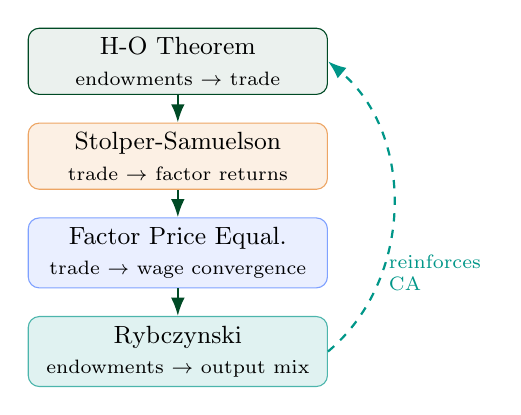
\begin{tikzpicture}[node distance=0.42cm,
  th/.style={draw=UNBCDark,fill=UNBCDark!8,rounded corners=4pt,
             minimum width=3.8cm,minimum height=0.62cm,
             align=center,font=\small}]
  \node[th](HO){H-O Theorem\\{\scriptsize endowments $\to$ trade}};
  \node[th,below=0.35cm of HO,fill=AccentOrange!12,
        draw=AccentOrange!70]
       (SS){Stolper-Samuelson\\{\scriptsize trade $\to$ factor returns}};
  \node[th,below=0.35cm of SS,fill=AccentBlue!10,
        draw=AccentBlue!60]
       (FPE){Factor Price Equal.\\{\scriptsize trade $\to$ wage convergence}};
  \node[th,below=0.35cm of FPE,fill=AccentTeal!12,
        draw=AccentTeal!70]
       (RY){Rybczynski\\{\scriptsize endowments $\to$ output mix}};
  \draw[-{Latex},UNBCDark,thick](HO)--(SS);
  \draw[-{Latex},UNBCDark,thick](SS)--(FPE);
  \draw[-{Latex},UNBCDark,thick](FPE)--(RY);
  \draw[-{Latex},AccentTeal,dashed,thick](RY.east)
       to[bend right=50](HO.east);
  \node[font=\scriptsize,AccentTeal,right=0.05cm of RY.east,
        anchor=west,text width=1.2cm,align=left]
       at ($(RY.east)+(0.6,1.0)$) {reinforces\\CA};
\end{tikzpicture}
\end{center}
\end{column}
\begin{column}{0.47\textwidth}
\small
The four theorems work together:
\begin{itemize}
  \item \textbf{H-O} predicts \emph{who} trades \emph{what}.
  \item \textbf{SS} predicts who \emph{gains} and who
        \emph{loses} --- the political economy of trade.
  \item \textbf{FPE} predicts the long-run equilibrium
        for wages if trade is truly free.
  \item \textbf{Rybczynski} predicts how factor
        accumulation and immigration change the
        \emph{production mix} and reinforce comparative
        advantage.
\end{itemize}
\vspace{0.3em}
Together they form the most complete general-equilibrium
model of trade we have studied.
\end{column}
\end{columns}
\end{frame}

%% ─────────────────────────────────────────────────────────────
%% 31. POLICY DEBATE: FOR AND AGAINST FREE TRADE
%% ─────────────────────────────────────────────────────────────
\begin{frame}[shrink=5]{Policy Debate: Why Do Countries Restrict Trade?}
\begin{columns}[T]
\begin{column}{0.52\textwidth}
\textbf{H-O makes a compelling case for free trade:}
\begin{itemize}\small
  \item Both countries gain in aggregate (larger
        consumption set).
  \item Abundant factors gain in real terms.
  \item Global resource allocation improves.
\end{itemize}
\vspace{0.3em}
\textbf{Yet governments routinely restrict trade.}\\
H-O itself explains \emph{why}:
\begin{itemize}\small
  \item SS: scarce factor owners lose from trade.
  \item Scarce factors lobby for protection
        (concentrated, organized interests).
  \item Gains are diffuse; losses are concentrated.
\end{itemize}
\vspace{0.3em}
\textbf{The politics:}\\
A few thousand steelworkers in Hamilton are a visible,
organized lobby. Two million Canadian consumers each
lose a few dollars from steel tariffs --- they do not
organize.
\end{column}
\begin{column}{0.45\textwidth}
\begin{canadex}[Steel Tariffs: SS in Practice]
\small In 2018, the US imposed Section 232 tariffs
on Canadian steel and aluminum (25\% and 10\%
respectively).\\[0.2em]
\textbf{SS winners}: Canadian steelworkers (capital
specific to steel protected) and steel producers.\\[0.2em]
\textbf{SS losers}: Canadian auto sector (input costs
rose), consumers (higher prices), US consumers
(welfare loss).\\[0.2em]
\textbf{Retaliation}: Canada imposed matching
counter-tariffs on US goods.\\[0.2em]
Tariffs were lifted in May 2019. Net welfare
effect: negative for both sides. Consistent
with SS but also with political-economy logic.
\end{canadex}
\end{column}
\end{columns}
\end{frame}

%% ─────────────────────────────────────────────────────────────
%% 32. CONNECTING TO INTERNATIONAL MACROECONOMICS
%% ─────────────────────────────────────────────────────────────
\begin{frame}[shrink=15]{Connecting to International Macroeconomics}
\begin{columns}[T]
\begin{column}{0.52\textwidth}
\textbf{H-O and the macro transmission chain for Canada:}
\begin{enumerate}\small
  \item \textbf{Resource endowment} (H-O): Canada exports
        oil, wheat, potash; China exports manufactures.
  \item \textbf{Oil price boom} (terms of trade):
        $P_{oil}\uparrow \Rightarrow$ Canadian ToT improves
        $\Rightarrow$ real income rises.
  \item \textbf{Rybczynski}: capital floods into Alberta
        oil sands; manufacturing contracts in Ontario.
  \item \textbf{Exchange rate}: CAD appreciates (more
        demand for Canadian dollars to buy oil exports).
  \item \textbf{Monetary policy}: Bank of Canada cannot
        cut rates (inflation in Alberta) and cannot
        raise rates (recession in Ontario) simultaneously.
  \item \textbf{NX}: $(X-M)$ rises initially; then Dutch
        Disease erodes manufactured exports.
\end{enumerate}
\end{column}
\begin{column}{0.45\textwidth}
\begin{varbox}
\small\textbf{H-O in the macro framework:}\\[0.3em]
$Y = C + I + G + \underbrace{(X-M)}_{NX}$\\[0.3em]
Trade pattern (H-O) determines the \emph{composition}
of NX: Canada's NX is positive in resources and
negative in manufactured goods.\\[0.3em]
Factor price effects (SS) shape the \emph{income
distribution} --- who can consume how much.\\[0.3em]
Rybczynski governs how factor accumulation
shifts NX over time.
\end{varbox}
\vspace{0.3em}
\begin{insight}{The Big Picture}
\small H-O is not just about \emph{what} a country
trades. It determines the structure of national
income, wages, and the external balance ---
all of which feed into macroeconomic policy.
\end{insight}
\end{column}
\end{columns}
\end{frame}

%% ─────────────────────────────────────────────────────────────
%% 33. FURTHER READING AND REFERENCES
%% ─────────────────────────────────────────────────────────────
\begin{frame}[shrink=12]{Key Empirical Papers and Further Reading}
\begin{columns}[T]
\begin{column}{0.50\textwidth}
\textbf{Foundational papers:}
\begin{itemize}\small
  \item Heckscher, E.\ (1919), ``The Effect of Foreign
        Trade on the Distribution of Income,''
        \textit{Ekonomisk Tidskrift}.
  \item Ohlin, B.\ (1933), \textit{Interregional and
        International Trade}, Harvard Press.
  \item Samuelson, P.\ (1948), ``International Trade
        and the Equalisation of Factor Prices,''
        \textit{EJ}.
  \item Stolper, W.\ \& Samuelson, P.\ (1941),
        ``Protection and Real Wages,'' \textit{RES}.
  \item Rybczynski, T.\ (1955), ``Factor Endowment
        and Relative Commodity Prices,''
        \textit{Economica}.
\end{itemize}
\end{column}
\begin{column}{0.47\textwidth}
\textbf{Empirical tests and extensions:}
\begin{itemize}\small
  \item Leontief, W.\ (1953), ``Domestic Production
        and Foreign Trade,'' \textit{PAPS}.
  \item Trefler, D.\ (1995), ``The Case of the
        Missing Trade,'' \textit{AER}, 85(5).
  \item Autor, D., Dorn, D., \& Hanson, G.\ (2013),
        ``The China Syndrome,'' \textit{AER}.
  \item Autor, D., Dorn, D., \& Hanson, G.\ (2016),
        ``The China Shock,''
        \textit{Annual Review of Economics}.
\end{itemize}
\vspace{0.3em}
\begin{varbox}
\footnotesize\textbf{Canadian applications:}\\
Statistics Canada, Labour Force Survey (wage data)\\
Bank of Canada Working Papers on Dutch Disease\\
C.D.\ Howe Institute analyses of CUSMA and supply
management
\end{varbox}
\end{column}
\end{columns}
\end{frame}

%% ─────────────────────────────────────────────────────────────
%% 34. DISCUSSION QUESTIONS
%% ─────────────────────────────────────────────────────────────
\begin{frame}[shrink=15]{Discussion Questions}
\begin{columns}[T]
\begin{column}{0.50\textwidth}
\begin{discuss}
\footnotesize
\begin{enumerate}
  \item Is Canada capital-abundant relative to Mexico?
        China? The US? How does your answer predict
        different trade patterns with each?
  \item Rybczynski says capital accumulation hurts
        the labour-intensive sector. Was Alberta's
        oil boom bad for Ontario workers?
  \item FPE predicts wages should equalize. Why don't
        Canadian labour unions treat this as a
        certainty?
  \item SS says trade lowers real wages for scarce
        factors. Should Canada restrict imports from
        China? What is the efficiency trade-off?
\end{enumerate}
\end{discuss}
\end{column}
\begin{column}{0.47\textwidth}
\begin{varbox}
\small\textbf{Exam-style warm-up:}\\[0.3em]
\textbf{(a)} Home: $K=300$, $L=300$.
Foreign: $K=100$, $L=300$.
Good $C$ ($a_K=6$, $a_L=3$) vs.
Good $T$ ($a_K=2$, $a_L=4$).\\[0.2em]
\begin{enumerate}
  \item Which country is capital-abundant?
  \item Which good is capital-intensive?
  \item Predict the trade pattern.
  \item After trade opens, what happens to real wages
        in Home?
\end{enumerate}
(This is Quiz~3 from Fall~2025.)
\end{varbox}
\end{column}
\end{columns}
\end{frame}

%% ─────────────────────────────────────────────────────────────
%% 35. LOOKING AHEAD
%% ─────────────────────────────────────────────────────────────
\begin{frame}[shrink=15]{Looking Ahead: From H-O to the Standard Trade Model}
\begin{columns}[T]
\begin{column}{0.52\textwidth}
\textbf{What H-O gives us:}
\begin{itemize}\small
  \item Complete GE model: factor endowments drive trade.
  \item Four theorems on trade, prices, and production.
  \item Framework for distributional analysis and
        political economy.
\end{itemize}
\vspace{0.2em}
\textbf{What H-O cannot do:}
\begin{itemize}\small
  \item Does not explain intra-industry trade
        (Canada exports \emph{and} imports cars).
  \item Abstracts from economies of scale.
  \item No welfare analysis of tariffs with
        terms-of-trade effects.
\end{itemize}
\end{column}
\begin{column}{0.45\textwidth}
\begin{varbox}
\small\textbf{Chapter~6: Standard Trade Model}\\[0.4em]
\textbf{Unifies} Ricardian, Specific Factors, and H-O
as special cases.\\[0.3em]
Introduces:
\begin{itemize}
  \item RS/RD framework for world price determination.
  \item Terms-of-trade welfare analysis.
  \item Export-biased vs.\ import-biased growth.
  \item Immiserizing growth (Bhagwati).
  \item Prebisch-Singer hypothesis.
\end{itemize}
\end{varbox}
\vspace{0.4em}
\begin{insight}{Preview Question}
\small If Canada's oil sector expands rapidly
(Rybczynski), and this lowers the world price of
oil (Canada's export), could Canada end up
\emph{worse off} despite growing richer?
That is immiserizing growth.
\end{insight}
\end{column}
\end{columns}
\end{frame}

%% ─────────────────────────────────────────────────────────────
%% 36. KEY EQUATIONS REFERENCE
%% ─────────────────────────────────────────────────────────────
\begin{frame}[shrink=8]{Key Equations: Chapter~5 Reference Sheet}
\begin{columns}[T]
\begin{column}{0.50\textwidth}
\textbf{Factor abundance:}
\[\tfrac{K_H}{L_H} > \tfrac{K_F}{L_F}
  \;\Rightarrow\; H\text{ is capital-abundant}\]
\textbf{Factor intensity (Cobb-Douglas):}
\[\tfrac{K_i}{L_i} = \tfrac{\alpha_i}{1-\alpha_i}
  \cdot\tfrac{w}{r}; \quad
  \tfrac{K_X}{L_X} > \tfrac{K_Y}{L_Y}
  \Rightarrow X\text{ is K-intensive}\]
\textbf{H-O theorem:}
$(K/L)_H > (K/L)_F \Rightarrow$
Home exports $X$ (K-intensive).\\[0.3em]
\textbf{Zero-profit conditions:}
\[\begin{aligned}
P_X &= a_{LX}\,w + a_{KX}\,r\\
P_Y &= a_{LY}\,w + a_{KY}\,r
\end{aligned}\]
\end{column}
\begin{column}{0.47\textwidth}
\textbf{Stolper-Samuelson magnification:}
\[\hat{r} > \hat{P}_X > 0 > \hat{P}_Y > \hat{w}\]
\small(if $X$ is K-intensive and $P_X\uparrow$)\\[0.3em]
\normalsize\textbf{Factor price equalization:}\\
\small Same tech + free trade $\Rightarrow$
$w^H = w^F$, $r^H = r^F$\\[0.3em]
\normalsize\textbf{Rybczynski:}
\[K\uparrow \;\Rightarrow\; Q_X\uparrow\uparrow,\;
  Q_Y\downarrow
  \quad\text{(at constant prices)}\]
\textbf{Rybczynski line:}
\[\tfrac{dQ_Y}{dQ_X}\bigg|_{\text{Ryb}} < 0\]
\small(one good rises, the other falls)
\end{column}
\end{columns}
\end{frame}

%% ─────────────────────────────────────────────────────────────
%% 37. KEY TAKEAWAYS
%% ─────────────────────────────────────────────────────────────
\begin{frame}[shrink=5]{Key Takeaways}
\begin{enumerate}\small
  \item \textbf{H-O Theorem}: countries export goods that use
        their abundant factor intensively. Factor endowments
        drive comparative advantage when technology is
        identical.
  \item \textbf{Stolper-Samuelson}: trade raises the real
        return to the abundant factor and lowers it for
        the scarce factor --- in terms of \emph{both} goods
        (magnification effect).
  \item \textbf{Factor Price Equalization}: free trade in
        goods can equate factor prices internationally without
        factor migration. Requires identical technology and
        no barriers --- too strong for the real world.
  \item \textbf{Rybczynski}: at constant prices, adding a factor
        expands the intensive sector and \emph{contracts} the
        other. Dutch Disease is Rybczynski in practice.
  \item \textbf{Leontief Paradox}: H-O performs better once
        we expand ``capital'' to include human capital and
        technology differences.
  \item \textbf{Trade and Inequality}: both trade (SS) and
        skill-biased technical change raise the skill premium;
        the China Shock shows trade effects are larger than
        previously estimated.
  \item \textbf{Canada}: resource abundance shapes comparative
        advantage; Dutch Disease and SS both explain Canadian
        regional and wage dynamics.
\end{enumerate}
\begin{block}{Next: Chapter~6 --- The Standard Trade Model}
A general synthesis of all models studied so far.
\end{block}
\end{frame}

\end{document}
